6. $(x+4)(3y-6x+9)=0\Leftrightarrow\left[\begin{array}{c}x+4=0,\\ 3y-6x+9=0.\end{array}
ight.\Leftrightarrow\left[\begin{array}{c}x=-4,\\ y=2x-3.\end{array}
ight.$
$$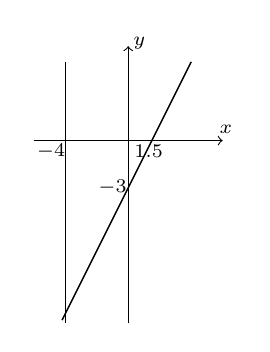
\begin{tikzpicture}[scale=0.2]
\tikzset {line01/.style={line width =0.5pt}}
\tikzset{line02/.style={line width =1pt}}
\tikzset{line03/.style={dashed,line width =0.5pt}}
%\filldraw [black] (0,0) circle (1pt);
\draw [->] (-6,0) -- (6,0);
\draw [->] (0,-11.6) -- (0,6);
\draw[line01] (-4,-11.6) -- (-4,5);
\draw[line01] (4,5) -- (-4.2,-11.4);
\draw (6.2,0.7) node {\scriptsize $x$};
\draw (-4.9,-0.7) node {\scriptsize $-4$};
\draw (1.3,-0.7) node {\scriptsize $1.5$};
\draw (-1,-3) node {\scriptsize $-3$};
\draw (0.7,6.2) node {\scriptsize $y$};
\end{tikzpicture}$$
